\documentclass[10pt,twocolumn]{article}
\usepackage[letterpaper,margin=0.65in]{geometry}
\usepackage{amsmath,amssymb,mathtools,bm}
\usepackage{graphicx}
\usepackage[T1]{fontenc}
\usepackage{lmodern}
\usepackage{xcolor}
\usepackage[normalem]{ulem}
\newcommand{\rev}[1]{\textcolor{red}{#1}}
\newcommand{\del}[1]{\textcolor{red}{\sout{#1}}}
\newenvironment{revision}{\color{red}}{}
\newcommand{\bAd}{\mathbf{Ad}}
\newcommand{\bad}{\mathbf{ad}}
\newcommand{\JopL}{\mathcal J_L}
\newcommand{\JopR}{\mathcal J_R}
\newcommand{\JL}{J_L}
\newcommand{\JR}{J_R}
\newcommand{\Exp}{\operatorname{Exp}}
\newcommand{\Log}{\operatorname{Log}}
\usepackage[hidelinks]{hyperref}
\usepackage{enumitem}
\setlength{\columnsep}{0.28in}
\setlength{\parindent}{1.2em}
\setlength{\parskip}{0pt}
\renewcommand{\thesection}{\Roman{section}}
\renewcommand{\thesubsection}{\thesection.\arabic{subsection}}
\newcommand{\SO}{\mathrm{SO}}
\newcommand{\SE}{\mathrm{SE}}
\newcommand{\so}{\mathfrak{so}}
\newcommand{\se}{\mathfrak{se}}
\newcommand{\gfrak}{\mathfrak g}
\newcommand{\Ad}{\operatorname{Ad}}
\newcommand{\ad}{\operatorname{ad}}
\newcommand{\tr}{\operatorname{tr}}
\newcommand{\R}{\mathbb R}
\newcommand{\idg}{\operatorname{id}_{\gfrak}}
\newcounter{paperitem}
\renewcommand{\thepaperitem}{\arabic{paperitem}}
\newcommand{\paperhead}[3]{\refstepcounter{paperitem}\par\medskip\noindent\textit{#1}\label{#3} #2\par}
\newcommand{\proofbox}{\hfill$\blacksquare$}

% Transcription policy:
% The rendered content follows the 7-page version, with only necessary mathematical
% and notation corrections adopted from the longer 47-page report. Ordinary wording,
% organization, theorem numbering, and the short-version bibliography are retained.

% Image dependencies from the previously prepared single-column version:
%   figures/fig1.png  = original single-column Figure~\ref{fig:proportional-actions-se2} (two panels)
%   figures/fig2.png  = original single-column Figure~\ref{fig:simulations-control-laws} (left double-geodesic, right logarithmic)
%   figures/fig3.png  = original single-column Figure 3 (left right-invariant double-geodesic, right logarithmic)
% This short version uses fig1 directly. Its Figure~\ref{fig:simulations-control-laws} is assembled by clipping panels from fig2 and fig3.

\title{Proportional Derivative (PD) Control on the Euclidean Group\thanks{An abbreviated version of this paper can be found in the Proc. of the 1995 European Control Conference.}}
\author{\begin{tabular}{cc}
Francesco Bullo\thanks{Work performed in part while author was with the Dipartimento di Ingegneria Elettronica, Universit\`a di Padova, Italy.} & Richard M. Murray\\
\texttt{bullo@indra.caltech.edu} & \texttt{murray@indra.caltech.edu}
\end{tabular}\\[1em]
Division of Engineering and Applied Science\\
California Institute of Technology\\
Pasadena, CA 91125}
\date{}

\begin{document}
\maketitle

% ECC'95-style compact body: in the 10pt article class, \small is 9pt with an 11pt baseline.
% This is the only pagination-oriented change; mathematical/text content below is unchanged.
% \small

\noindent\textbf{Keywords:} PD control, Euclidean group, nonlinear control, workspace control

\begin{abstract}
In this paper we study the stabilization problem for control systems defined on $\SE(3)$, the Euclidean group of rigid-body motions. Assuming one actuator is available for each degree of freedom, we exploit geometric properties of Lie groups (and corresponding Lie algebras) to generalize the classical PD control in a coordinate-free way. For the $\SO(3)$ case, the compactness of the group gives rise to a natural metric structure and to a natural choice of preferred control direction: an optimal (in the sense of geodesic) solution is given to the attitude control problem. In the $\SE(3)$ case, no natural metric is uniquely defined, so that more freedom is left in the control design. Different formulations of PD feedback can be adopted by extending the $\SO(3)$ approach to the whole of $\SE(3)$ or by breaking the problem into a control problem on $\SO(3)\times\R^3$. For the simple $\SE(2)$ case, simulations are reported to illustrate the behavior of the different choices. Finally, we discuss the trajectory tracking problem and show how to reduce it to a stabilization problem, mimicking the usual approach in $\R^n$.
\end{abstract}

\section{Introduction}\label{sec:introduction}
We here consider the problem of controlling a (mechanical) system whose configuration space is a matrix Lie group: we focus on second order systems and attempt to generalize the standard notion of proportional derivative feedback. One large class of applications which motivates this work is workspace control of robotic manipulators, where the end-effector configuration is naturally embedded in $\SE(3)$ (see \cite{1} for a description of the workspace control problem and traditional solutions). While local solutions are easily obtained, we hope that a more geometric approach will yield advantages similar to those afforded by the geometric approach to kinematics in \cite{1}.

Historically, nonlinear control systems defined on Lie groups have received considerable attention in the literature: early work by Brockett \cite{2,3}, and others has served as motivation for more recent contributions by Walsh, Sarti, Sastry and Montgomery \cite{4,5}, Leonard and Krishnaprasad \cite{6}, and Crouch and Silva Leite \cite{7}, to name a few. Early works concentrated on problem formulation and controllability issues, while the more recent papers mainly consider constructive controllability: how to generate a feasible trajectory between two (or more) points on the configuration manifold given a limited number of actuators.

Our approach in this paper is somewhat different. We concentrate on the problems of stabilization and trajectory tracking in the fully actuated case, where one actuator is available for each degree of freedom in the system. This is traditionally the situation for problems in robotic manipulation, satellite reorientation and 6 degree of freedom underwater vehicles. We attempt to exploit the geometric properties of Lie groups and to generalize the classical proportional plus derivative feedback (PD) used for control of simple mechanical systems in $\R^n$. For the case of compact Lie groups, such as $\SO(3)$, our results are completely general. For the non-compact case, we consider only control systems on $\SE(3)$ and on its subgroups, since those are the main systems of interest in our applications.

The paper is organized as follows. In Section~\ref{sec:systems-lie-groups}, we introduce basic and new results on systems defined on Lie groups. Section~\ref{sec:pd-so3} shows stabilization results for the compact case and in particular for $\SO(3)$. Section~\ref{sec:pd-se3} considers the $\SE(3)$ case, a non-compact non-semisimple group. Different metrics lead to different control laws. These results are then generalized to the trajectory tracking case in Section~\ref{sec:trajectory-tracking}. Section~\ref{sec:discussion} discusses the results and the underactuated case. For all the proofs and for a more detailed version of this paper we refer to \cite{8}.

\section{Systems on Lie groups}\label{sec:systems-lie-groups}
We here review the notations and give some algebraic results on Lie groups and on dynamical systems evolving on Lie groups. For a comprehensive introduction see \cite{1}.

\subsection{Basic definitions and results}\label{subsec:basic-definitions}
In the following we focus our attention on the matrix Lie group $\SE(3)$ and its proper subgroups, even though most of the results hold more generally. Let $G\subset\SE(3)$ be a matrix Lie group and $\gfrak\subset\se(3)$ its Lie algebra. A dynamical system with state $g\in G$ evolves following
\begin{equation*}
\dot g=gV^b=V^s g,\qquad V^b,V^s\in\gfrak.\tag{1}\label{eq:1}
\end{equation*}
where we can express the velocity in body ($V^b$) or in spatial frame ($V^s$). Since the system $\dot g=gV^b$ is invariant under left multiplications by constant matrices, we call it \emph{left invariant}; correspondingly $\dot g=V^s g$ is said to be \emph{right invariant}. For all $g\in G$ and all $X,Y\in\gfrak$, the adjoint map $\Ad_g$ and the matrix commutator $\ad_X$ are defined as
\begin{equation*}
\Ad_g(Y)=gYg^{-1},
\qquad
\ad_X(Y)=[X,Y]=XY-YX.
\end{equation*}
\begin{revision}
\noindent\textbf{Notation bridge to modern Lie-group robotics conventions.}
The symbols $\Ad_g:\gfrak\to\gfrak$ and $\ad_X:\gfrak\to\gfrak$ retain their original
meaning as basis-free linear maps.  After choosing a basis $\mathcal E=(E_1,\ldots,E_n)$ of
$\gfrak$, write
\[
X=x^\wedge=\sum_{i=1}^n x_iE_i,\qquad x=X^\vee,
\]
and denote the corresponding matrices by
\[
\bAd_g:=\vee\circ\Ad_g\circ\wedge,\qquad
\bad_x:=\vee\circ\ad_{x^\wedge}\circ\wedge.
\]
When a coordinate-valued exponential or logarithm is useful, we write
\[
\Exp(x):=\exp(x^\wedge),\; \Log(g):=(\log g)^\vee,
\]
\[
\Log_{\SO(3)}(R):=(\log_{\SO(3)}R)^\vee.
\]
The original manuscript's $\exp/\log$ notation is otherwise retained; an occurrence is
changed to $\Log$ only when the surrounding formula is explicitly coordinate-valued and the
original $\log$ therefore relies on the implicit hat/vee identification.  For $\SE(3)$ coordinate vectors and their matrix representations, this annotated version
retains the rotation--translation ordering used in the original manuscript,
\[
x=X^\vee=\begin{bmatrix}\psi\\q\end{bmatrix},\qquad
\nu=V^\vee=\begin{bmatrix}\omega\\v\end{bmatrix}.
\]
Thus the ordered pairs $X=(\widehat\psi,q)$ and $V=(\widehat\omega,v)$, their coordinate
vectors, and the associated matrix representations all use the same ordering.
\end{revision}

On $\SE(3)$ and $\se(3)$ we represent a group element $g=(R,p)\in\SO(3)\times\R^3$ and a velocity $V=(\widehat\omega,v)\in\so(3)\times\R^3$ using homogeneous coordinates,
\begin{equation*}
g=\begin{bmatrix}R&p\\0&1\end{bmatrix},
\qquad
V=\begin{bmatrix}\widehat\omega&v\\0&0\end{bmatrix},
\end{equation*}
where the operator $\widehat{\phantom{x}}:\R^3\to\so(3)$ is defined so that $\widehat{x}y=x\times y$ for all $x,y\in\R^3$.
\begin{revision}
With the original rotation--translation coordinate ordering $\nu=V^\vee=[\omega^T\ v^T]^T$, the matrix representations corresponding to the abstract maps above are
\[
\bAd_g=\begin{bmatrix}R&0\\\widehat pR&R\end{bmatrix},\qquad
\bad_\nu=\begin{bmatrix}\widehat\omega&0\\\widehat v&\widehat\omega\end{bmatrix}.
\]
\end{revision}


On $\SE(3)$ and on its proper subgroups the exponential map $\exp:\gfrak\to G$ is a surjective map and a local diffeomorphism. Standard computations show:

\paperhead{Lemma 1.}{(Exponential Map) Given $\widehat\psi\in\so(3)$ and $X=(\widehat\psi,\rev{q})\in\se(3)$,}{lem:exp-map}
\begin{revision}
The short version used $p$ both for the group translation and for this translational
Lie-algebra coordinate.  The latter is denoted $q$ here, matching the full technical report
and removing that local ambiguity.
\end{revision}
\begin{align*}
\exp_{\SO(3)}(\widehat\psi)
&=I+\frac{\sin\|\psi\|}{\|\psi\|}\widehat\psi
+\frac{1-\cos\|\psi\|}{\|\psi\|^2}\widehat\psi^2,\\[0.4em]
\exp_{\SE(3)}(X)
&=\begin{bmatrix}
\exp_{\SO(3)}(\widehat\psi)&A(\psi)\rev{q}\\
0&1
\end{bmatrix},
\end{align*}
where $\|\psi\|$ is the standard Euclidean norm and
\begin{equation*}
A(\psi)=I+\frac{1-\cos\|\psi\|}{\|\psi\|^2}\widehat\psi
+\frac{\|\psi\|-\sin\|\psi\|}{\|\psi\|^3}\widehat\psi^2.
\end{equation*}
\begin{revision}
The original symbol $A(\psi)$ is retained.  With the left/right Jacobian convention used
in this annotated edition, this particular $\SE(3)$ translational exponential factor satisfies
\[
A(\psi)=J_L^{\SO(3)}(\psi),\qquad
A(\psi)^{-T}=J_R^{\SO(3)}(\psi)^{-1}.
\]
Sol\`a denotes the same translational factor by $V(\psi)$; that additional symbol is not
adopted here because $V,V^b,V^s$ already denote velocities in the original manuscript.
\end{revision}

In an open neighborhood of the origin dense in $G$, we define $X=\log(g)\in\gfrak$ to be the \emph{exponential coordinates} of the group element $g$ and we regard the logarithmic map as a local chart of the manifold $G$.
\begin{revision}
Thus $\log(g)\in\gfrak$ denotes the Lie-algebra element exactly as in the original text; when
its coordinate vector is intended we write $x=\Log(g)=(\log g)^\vee$.
\end{revision}


\paperhead{Lemma 2.}{(Logarithmic map) Given $(R,p)\in\SO(3)\times\R^3$ such that $\tr(R)\neq-1$. Then}{lem:log-map}
\begin{equation*}
\log_{\SO(3)}(R)=\frac{\phi}{2\sin\phi}(R-R^T)\in\so(3),
\end{equation*}
where $\phi$ satisfies $\cos\phi=(\tr(R)-1)/2$ and $|\phi|<\pi$. Also
\begin{equation*}
\log_{\SE(3)}(R,p)=
\begin{bmatrix}
\widehat\psi&A^{-1}(\psi)p\\
0&1
\end{bmatrix}\in\se(3),
\end{equation*}
where $\widehat\psi=\log_{\SO(3)}(R)$ and
\begin{equation*}
A^{-1}(\psi)=I-\frac12\widehat\psi
+\frac{2\sin\|\psi\|-\|\psi\|(1+\cos\|\psi\|)}{2\|\psi\|^2\sin\|\psi\|}\widehat\psi^2.
\end{equation*}

Note that elements of the Lie algebra $\gfrak$ can represent a velocity as in equation~\eqref{eq:1} or can represent the matrix logarithm of the state (and should therefore be considered states) as in Lemma~\ref{lem:log-map}. We denote them with $V=(\widehat\omega,v)$ in the first case and with $X=(\widehat\psi,\rev{q})$ in the second.

\subsection{The Jacobian of the exponential map}\label{subsec:jacobian-exponential}
We now want to compute explicit formulas that relate the time derivative of $X(t)=\log(g(t))$ with the body and spatial velocities $V^b,V^s$. Indeed only for the linear time dependence case ($X(t)=Yt$), it is easy to show that $\dot X=Y=V^b=V^s$; for the generic case $X=X(t)$ the relationship is not trivial.

\paperhead{Theorem 3.}{(Differential of Exponential) Let $g(t)$ be a smooth curve on $G$, $X(t)=\log(g(t))$ be the exponential coordinates of $g(t)$, $V^b=g^{-1}\dot g$ the body velocity and $V^s=\dot g g^{-1}$ the spatial velocity. Then it holds}{thm:differential-exponential}
\begin{align*}
\dot X&=\sum_{n=0}^{\infty}\frac{(-1)^nB_n}{n!}\ad_X^n(V^b)\\
&=\sum_{n=0}^{\infty}\frac{B_n}{n!}\ad_X^n(V^s),
\end{align*}
where $\{B_n\}$ are the Bernoulli numbers.
\begin{revision}
For compatibility with later left/right-Jacobian notation, the two basis-free inverse
differentials represented by Theorem~\ref{thm:differential-exponential} are denoted
\[
\JopR^{-1}(X)
:=\sum_{n=0}^{\infty}\frac{(-1)^nB_n}{n!}\ad_X^n,
\;
\JopL^{-1}(X)
:=\sum_{n=0}^{\infty}\frac{B_n}{n!}\ad_X^n.
\]
After choosing a basis,
\[
\JR^{-1}(x)=\sum_{n=0}^{\infty}\frac{(-1)^nB_n}{n!}\bad_x^n,
\qquad
\JL^{-1}(x)=\sum_{n=0}^{\infty}\frac{B_n}{n!}\bad_x^n,
\]
so the theorem is equivalently
\[
\dot x=\JR^{-1}(x)\nu^b=\JL^{-1}(x)\nu^s,
\qquad \nu^{b,s}:=(V^{b,s})^\vee.
\]
\end{revision}

In the pure rotation case, summing the series we obtain:

\paperhead{Lemma 4.}{(Exponential coordinates on $\SO(3)$) Let $R(t)$ be a smooth curve on $\SO(3)$, $\widehat{x}(t)=\log(R(t))$ be the exponential coordinates of $R(t)$ and $\widehat\omega=R^{-1}\dot R$ the body angular velocity. Then we have}{lem:so3-exponential-coordinates}
\begin{equation*}
\dot x=\omega_{\parallel}+\beta(\|x\|)\omega_{\perp}+\frac12(x\times\omega)
\end{equation*}
where $\beta(y)\triangleq\dfrac{y/2}{\tan(y/2)}$ and $\omega=\omega_{\parallel}+\omega_{\perp}$ is the orthogonal decomposition of $\omega$ along $\operatorname{span}\{x\}$ and $\operatorname{span}\{x\}^{\perp}$.
\begin{revision}
With $x=\Log(R)$, this is the standard inverse-right-Jacobian relation
\[
\dot x=J_R^{\SO(3)}(x)^{-1}\omega.
\]
\end{revision}

To the authors' knowledge this expression is novel and relates the time derivative of the angle-axis quantity $x$ with the often used $\omega$. Similar expressions can be obtained for the $\SE(3)$ and $\SE(2)$ cases (for more details see \cite{8}).

\subsection{Metric properties on compact Lie groups}\label{subsec:metric-compact}
On any Lie group $G$, the Killing form $\langle\cdot,\cdot\rangle_K$ is defined as the bilinear operator on $\gfrak\times\gfrak$:
\begin{equation*}
\langle X,Y\rangle_K\triangleq\tr(\ad_X\cdot\ad_Y),\qquad \forall X,Y\in\gfrak.
\end{equation*}
A Lie group is said to be \emph{semi-simple} if $\langle\cdot,\cdot\rangle_K$ is nondegenerate. For \emph{compact} Lie groups $\langle\cdot,\cdot\rangle_K$ is both nondegenerate and negative definite, so that by a simple multiplication with a negative constant, we can define an inner product on the Lie algebra $\gfrak$ (e.g. on $\so(3)$ $\langle\cdot,\cdot\rangle\triangleq-1/4\langle\cdot,\cdot\rangle_K$). An inner product defined this way will satisfy the crucial property of \emph{Ad-invariance}:
\begin{equation*}
\langle X,Y\rangle=\langle\Ad_gX,\Ad_gY\rangle,\qquad \forall g\in G,
\end{equation*}
where $\Ad$ is therefore an orthogonal operator of $\gfrak$. Equivalently the matrix commutator satisfies
\begin{equation*}
\langle\ad_ZX,Y\rangle=-\langle X,\ad_ZY\rangle,
\qquad \forall Z\in\gfrak.\tag{2}\label{eq:2}
\end{equation*}

Now, an Ad-invariant inner product on the algebra $\gfrak$ induces an Ad-invariant metric on the group $G$ by either left or right translation: this gives the additional structure of Riemannian manifold to the group $G$. Without entering details, we refer to \cite{9} and we simply state the following result:



\paperhead{Proposition 5.}{With respect to an Ad-invariant metric, the geodesics of $G$ are the one parameter subgroups, that is the curves of the form $\exp(Yt)$, with $Y\in\gfrak$ constant. Furthermore, the distance between the element $g$ and the identity $e_G=I\in G$ is given by the norm of the logarithmic function:}{prop:geodesics}
\begin{equation*}
\|g\|_G=\langle\log(g),\log(g)\rangle^{1/2}.\tag{3}\label{eq:3}
\end{equation*}

The computational result we are interested in, is an extension of Gauss's Lemma (see \cite{9} and \cite{10}), obtained thanks to property~\eqref{eq:2} and equation~\eqref{eq:3}.

\paperhead{Theorem 6.}{(Derivative of distance function) Let $G$ be a compact Lie group with bi-invariant metric $\langle\cdot,\cdot\rangle$. Consider a smooth trajectory $g(t)\in G$, such that $g(t)$ never passes through a singularity of the exponential map. Then}{thm:distance-derivative}
\begin{equation*}
\frac12\frac{d}{dt}\|g\|_G^2=\langle\log(g),V^b\rangle=\langle\log(g),V^s\rangle.
\end{equation*}

\section{PD control on $\SO(3)$}\label{sec:pd-so3}
We begin with the problem of stabilizing a control system evolving on a compact, semisimple Lie group. Without loss of generality we will here consider only the $\SO(3)$ case. As explained in the previous section, a bi-invariant Riemannian metric is naturally defined on $\SO(3)$ and allow us to easily design appropriate Lyapunov functions.


We begin by briefly describing our approach for a simple \emph{first order system} on $\SO(3)$, described as in equation~\eqref{eq:1} by $\dot g=gV^b$. Consider the natural candidate Lyapunov function
\begin{equation*}
W(g)=\frac12\|g\|_{\SO(3)}^2,
\end{equation*}
and assume we can directly control the quantity $V^b\in\so(3)$ to any desired value (i.e. the system is fully actuated). Then the proportional control action
\begin{equation*}
V^b=-k_p\log(g),\qquad k_p>0,\tag{4}\label{eq:4}
\end{equation*}
leads to
\begin{equation*}
\dot W(g(t))=\langle\log(g),-k_p\log(g)\rangle=-2k_pW,
\end{equation*}
thanks to Theorem~\ref{thm:distance-derivative}. Thus, for this first order system, a logarithmic control law ensures exponential stability for all initial conditions $g(0)$ such that $\tr(g(0))\neq-1$.

Now, motivated by standard control problems in mechanics and robotics, we consider the stabilization problem for second order systems, that is for systems where we have full control over forces (accelerations) rather than velocities. A \emph{second order system on $\SO(3)$} has the form
\begin{equation*}
\left\{\begin{aligned}
\dot g&=gV^b,\\
\dot V^b&=f(g,V^b)+U,
\end{aligned}\right.\tag{5}\label{eq:5}
\end{equation*}
where $g\in\SO(3)$ is the configuration of the system, $f(g,V^b)\in\so(3)$ is the internal drift, and $U\in\so(3)$ is the control input. Note that we once again assume that the system is fully actuated. To regulate the state $g$ to the identity matrix $I\in\SO(3)$, we couple the proportional action~\eqref{eq:4} with a derivative term, i.e. with a term proportional to the velocity $V^b$.

\paperhead{Theorem 7.}{(PD Control on $\SO(3)$) Consider the system in equation~\eqref{eq:5} and let $K_p$ and $K_d$ be symmetric, positive definite gains. Then the control law}{thm:pd-so3}
\begin{equation*}
U=-f(g,V^b)-K_p\log(g)-K_dV^b,\tag{6}\label{eq:6}
\end{equation*}
exponentially stabilizes the state $g$ at $I\in\SO(3)$ from any initial condition $\tr(g(0))\neq-1$ and for all $K_p$ and $V^b(0)$ such that
\begin{equation*}
\lambda_{\min}(K_p)>\frac{\|V^b(0)\|^2}{\pi^2-\|g(0)\|_{\SO(3)}^2},
\end{equation*}
where $\lambda_{\min}(K_p)$ is the minimum eigenvalue of $K_p$.

\noindent\textit{Proof.} The stability analysis is based on the candidate Lyapunov function
\begin{equation*}
W=\frac12\left\langle
\begin{bmatrix}\log(g)\\V^b\end{bmatrix},
\begin{bmatrix}
\idg&\epsilon\idg\\
\epsilon\idg&K_p^{-1}
\end{bmatrix}
\begin{bmatrix}\log(g)\\V^b\end{bmatrix}
\right\rangle,
\end{equation*}
where the inner product is taken in $\so(3)\times\so(3)$ and $\epsilon$ is taken small enough. For the details we refer to \cite{8}. \proofbox


\paperhead{Remark 8.}{We have written the control law~\eqref{eq:4} and Theorem~\ref{thm:pd-so3} in terms of the body velocity $V^b$, i.e. we assumed ``body-fixed'' control inputs. A dual version can be easily written for the opposite case of ``spatial-fixed'' control inputs, i.e. for the case $\dot V^s=f(g,V^s)+U$. Thanks to Theorem~\ref{thm:distance-derivative} a logarithmic control law is the correct choice also for this case.}{rem:body-spatial-control}

\subsection{Example: orientation control of a satellite}\label{subsec:satellite-orientation}
The primary example of control problem on a compact Lie group is attitude control of a satellite.

In the literature, various PD control laws based on different parametrization of the manifold $\SO(3)$ have been proposed: Euler angles \cite{11}, Gibb's vectors \cite{12} and unit quaternions \cite{13}. In particular, Wen and Kreutz-Delgado \cite{13} introduce the idea that the ``error measure should correspond to the topology of the error space''. Here we additionally require that the error measure correspond to the (natural) metric of the Riemannian manifold $\SO(3)$. The second order model of a satellite is
\rev{To avoid collision with the newly introduced Lie Jacobians $J_L,J_R$, the rigid-body inertia tensor, denoted $J$ in the original manuscript, is denoted $\mathbb I$ in this annotated version.}\par
\begin{equation*}
\left\{\begin{aligned}
\dot g&=g\widehat\omega^b,\\
\rev{\mathbb I}\dot\omega^b&=f(g,\omega^b)+\tau,
\end{aligned}\right.
\end{equation*}
where the control inputs $\tau$ is the total torque applied to the satellite either by momentum wheels or by gas jet actuators. The internal drift is
\begin{equation*}
f(g,\omega^b)=
\begin{cases}
[g^Tm_0,\omega^b],&\text{momentum wheels},\\
[\rev{\mathbb I}\omega^b,\omega^b],&\text{gas jet (Euler equations)}.
\end{cases}
\end{equation*}
Following early work by Koditschek \cite{14}, we introduce a slight modification to the design of Theorem~\ref{thm:pd-so3} and we adopt the modified Lyapunov function
\begin{equation*}
W=\frac{k_p}{2}\|g\|_{\SO(3)}^2+\frac12\langle\omega^b,\rev{\mathbb I}\omega^b\rangle_{\R^3}
+\epsilon\langle\rev{\Log(g)},\rev{\mathbb I}\omega^b\rangle
\end{equation*}
where the second term has the strong interpretation of kinetic energy. This leads to the feedback law
\begin{equation*}
\tau=-k_p\rev{\Log(g)}-K_d\omega^b\tag{7}\label{eq:7}
\end{equation*}
where we write the control law in $\R^3$ making use of the isomorphism $\widehat{\phantom{x}}$ given in Section~\ref{sec:systems-lie-groups}.

This feedback has strong similarities to the ones already proposed in the literature: it is instructive to compare it with the equivalent proposed in \cite{13}. Both laws consist of the sum of a proportional and derivative action, where they differ is in the expression of the proportional term. In particular along the ``geodesic'' direction (equal to the rotation axis of the attitude matrix $g$), the two laws differ in the intensity of control action. Our feedback relies on the notion of group norm (as defined in equation~\eqref{eq:3}) and is proportional to this quantity. Instead the control laws proposed by Wen and Kreutz-Delgado are based on either the 2-norm of the unit quaternion or the 2-norm of the vector quaternion, and therefore exert an action proportional to either $\sin\|g\|$ or $2\sin(\|g\|/2)$.

\section{PD control on $\SE(3)$}\label{sec:pd-se3}
Another common Lie group in robotic applications is $\SE(3)$. Unfortunately, since this Lie group is not compact, the results of the previous section cannot be applied directly. As before, we begin by studying the simple first order case and we then couple proportional with derivative action for second order systems. Finally we apply our results to the case of mechanical manipulators and we then report some simulations.

\subsection{Proportional actions on $\SE(3)$ and first order systems}\label{subsec:proportional-se3}
The geometric properties of the group $\SE(3)$ have received much attention in the recent control literature \cite{3,1} and a very complete treatment is contained in \cite{15}. A well-known negative result is the following: no symmetric bilinear form on $\se(3)$ can be both positive-definite and Ad-invariant. There is therefore an algebraic obstruction to the procedure we have followed for the $\SO(3)$ case.

Recall the design procedure: we need a positive-definite bilinear form (hence an inner product) to construct a Lyapunov function $W$, and we need the Ad-invariance of this form to compute the time derivative of $W$ (Theorem~\ref{thm:distance-derivative}). Unfortunately the only bilinear forms on $\se(3)$ are the following. Let $V_i=(\omega_i,v_i)$ for $i=1,2$ and consider
\begin{itemize}[leftmargin=1.4em,label=$\square$,itemsep=0.25em,topsep=0.25em]
\item \textbf{a linear combination of Klein and Killing form:} the most generic Ad-invariant form on $\se(3)$ looks like
\begin{equation*}
\langle V_1,V_2\rangle_{\mathrm{Ad-inv}}
=\alpha\langle\omega_1,\omega_2\rangle
+\beta\bigl(\langle\omega_1,v_2\rangle+\langle\omega_2,v_1\rangle\bigr),
\end{equation*}
\item \textbf{the standard inner product on $\se(3)=\R^6$:} discard the Lie algebra structure of $\se(3)$ and write
\begin{equation*}
\langle V_1,V_2\rangle_{\R^6}
=\langle\omega_1,\omega_2\rangle+\langle v_1,v_2\rangle.\tag{8}\label{eq:8}
\end{equation*}
\end{itemize}
Hence we are left with two possible design choices: as proportional action we can insist on the logarithm function (this corresponds to giving up the positive-definiteness), or (giving up the Ad-invariance) we can still regard $\SE(3)$ as a metric space with respect to the inner product~\eqref{eq:8} and compute the correct proportional action within this new framework\footnote{Given an inner product on $\gfrak$, we can extend it to the whole $TG$ by either left or right translation: we end up therefore with a metric structure on $G$. We refer to \cite{9} for a detailed treatment of this standard construction.}. The two procedures are described in Figure~\ref{fig:proportional-actions-se2}; the following lemmas formalize this previous discussion.

\paperhead{Lemma 9.}{Consider the $\SE(3)$ system $\dot g=gV^b$ and let $k_p>0$. Then the control law}{lem:log-feedback-se3}
\begin{equation*}
V^b=-k_p\log(g)\tag{9}\label{eq:9}
\end{equation*}
exponentially stabilizes the state $g$ at $I$ with time constant $k_p$, from any initial condition $g(0)=(R(0),p(0))$ such that $\tr(R(0))\neq-1$.

The second approach is based on the decomposition of the control system on $\SE(3)$ into a control system on $\SO(3)\times\R^3$. Recall the notation introduced in Section~\ref{sec:systems-lie-groups}: $g=(R,p)$, $V^s=(\widehat\omega^s,v^s)$, $V^b=(\widehat\omega^b,v^b)$. The original systems $\dot g=gV^b$ and $\dot g=V^s g$ reduce to
\begin{equation*}
\left\{\begin{aligned}
\dot R&=R\widehat\omega^b,\\
\dot p&=Rv^b,
\end{aligned}\right.
\qquad\text{and}\qquad
\left\{\begin{aligned}
\dot R&=\widehat\omega^sR,\\
\dot p&=\omega^s\times p+v^s.
\end{aligned}\right.
\end{equation*}
Indeed adopting the bilinear form~\eqref{eq:8} involves applying a proportional action along geodesic directions for both the subsystems in $\SO(3)$ and $\R^3$ (see \cite{8} for more details).

\begin{figure}[t]
\centering
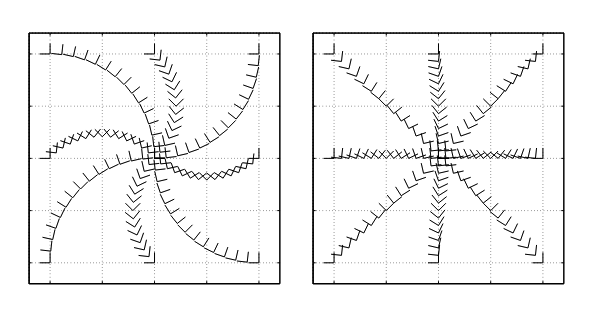
\includegraphics[width=\columnwidth]{figures/fig1_b.png}
\caption{Proportional actions on $\SE(2)$: on the left the logarithmic function, on the right double-geodesics for $\SO(2)\times\R^2$. Each point $g\in\SE(2)$ is depicted as a frame on the plane.}\label{fig:proportional-actions-se2}
\label{fig:short-proportional}
\end{figure}

\paperhead{Lemma 10.}{Consider the $\SE(3)$ system $\dot g=gV^b$ and let $K_v,K_\omega$ be positive definite symmetric gains. Then the control law}{lem:double-geodesic-feedback}
\begin{equation*}
\left\{\begin{aligned}
\omega^b&=-K_\omega\rev{\Log_{\SO(3)}(R)},\\
v^b&=-R^TK_vp,
\end{aligned}\right.
\end{equation*}
exponentially stabilizes the state $g$ at $I$, from any initial condition $g(0)=(R(0),p(0))$ such that $\tr(R(0))\neq-1$.

Similar versions of the two lemmas can be easily written for the right invariant case ($\dot g=V^s g$). Because of the basic Lie group identity $\Ad_g\log(g)=\log(g)$, it is easy to show that left and right invariant systems behave the same way under the logarithmic control law. This is not true for the double-geodesic law, as we shall see also in the simulations (again, see \cite{8} for more details).

\subsection{Second order systems}\label{subsec:second-order-se3}
We now apply these proportional strategies, coupled with a derivative term, to second order, fully actuated systems on $\SE(3)$. Consider the left invariant \emph{second order system on $\SE(3)$}:
\begin{equation*}
\left\{\begin{aligned}
\dot g&=gV^b,\\
\dot V^b&=f(g,V^b)+U,
\end{aligned}\right.\tag{10}\label{eq:10}
\end{equation*}
where $f(g,V^b),U\in\se(3)$ are internal drift and control input. The previous discussion leads to the two theorems:

\paperhead{Theorem 11.}{(Regulation via the logarithm function) Consider the system in equation~\eqref{eq:10} and let $k_p>0$ and $K_d=K_d^T>0$. Then the control law}{thm:log-regulation}
\begin{equation*}
U(g,V^b)=-f(g,V^b)-k_p\log(g)-K_dV^b,
\end{equation*}
locally exponentially stabilizes the state $g$ at $I\in\SE(3)$.

\paperhead{Theorem 12.}{(Regulation via the double-geodesic law) Consider the system in equation~\eqref{eq:10} and let $K_\omega,K_v$ and $K_d$ be the positive definite gains. Then the control law}{thm:double-geodesic-regulation}
\begin{equation*}
U(g,V^b)=-f(g,V^b)-
\begin{bmatrix}
K_\omega\rev{\Log_{\SO(3)}(R)}\\
R^TK_vp
\end{bmatrix}-K_dV^b,
\end{equation*}
exponentially stabilizes the state $g$ at $I$ from any initial condition $g(0)=(R(0),p(0))$ with $\tr(R(0))\neq-1$ and for all $K_\omega$ and $\omega^b(0)$ such that
\begin{equation*}
\lambda_{\min}(K_\omega)>\frac{\|\omega^b(0)\|^2}{\pi^2-\|R(0)\|_{\SO(3)}^2}.
\end{equation*}

\begin{figure*}[t]
\centering
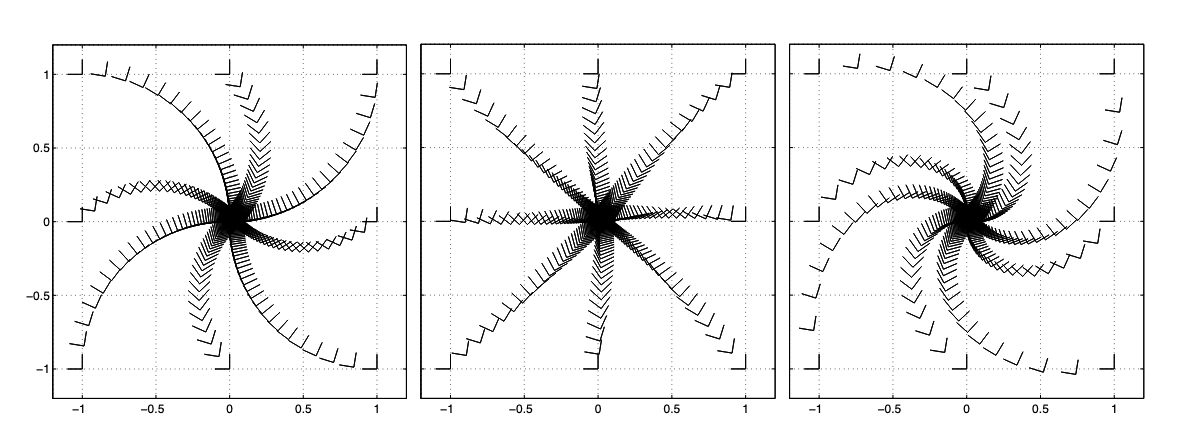
\includegraphics[width=0.8\textwidth]{figures/fig2_b.png}
\caption{Simulations of control laws in Theorems~\ref{thm:log-regulation},~\ref{thm:double-geodesic-regulation} and Remark~\ref{rem:right-invariant} for systems defined on $\SE(2)$. From left to right: left invariant system with logarithmic control law (Theorem~\ref{thm:log-regulation}), left invariant system with double-geodesic control law (Theorem~\ref{thm:double-geodesic-regulation}), right invariant system with double-geodesic control law (Remark~\ref{rem:right-invariant}).}\label{fig:simulations-control-laws}
\label{fig:short-simulations}
\end{figure*}

\paperhead{Remark 13.}{As usual we can extend to the right invariant case ($\dot g=V^s g$) all we have done for the left one. For both systems the logarithmic control law (in Theorem~\ref{thm:log-regulation}) is identical and it can be shown that the closed loop vector field is exactly the same. Instead, the double-geodesic law applied to a right system has the slightly different expression:}{rem:right-invariant}
\begin{equation*}
U(g,V^s)=-f(g,V^s)-
\begin{bmatrix}
K_\omega\rev{\Log_{\SO(3)}(R)}\\
K_vp
\end{bmatrix}-K_dV^s.
\end{equation*}

\subsection{Example: workspace control of robotic manipulators and 6 DOF underwater vehicles}\label{subsec:workspace-control}
As in Subsection~\ref{subsec:satellite-orientation}, we apply our control laws to mechanical systems. After a change of coordinates and inputs, 6 degree of freedom robotic manipulators and underwater vehicles can be modeled as
\begin{equation*}
\left\{\begin{aligned}
\dot g&=gV^b,\\
M(g)\dot V^b&=C(g,V^b)V^b+N(g,V^b)+U,
\end{aligned}\right.
\end{equation*}
where $M(g)$ is the inertia matrix, $C(g,V^b)$ is the Coriolis matrix and $N(g,V^b)$ are some generic extra terms. The kinetic energy of this mechanical system, is computed with the positive definite form~\eqref{eq:8} (coupled with the left translation of the velocity $gV^b$). Hence, for this class of systems, we are naturally lead to prefer the double-geodesic control law over the logarithmic one:
\begin{equation*}
U(g,V^b)=-N(g,V^b)-k_p
\begin{bmatrix}
\rev{\Log_{\SO(3)}(R)}\\
R^Tp
\end{bmatrix}-K_dV^b.
\end{equation*}
Exponential stability is proved through the Lyapunov function
\begin{align*}
W(g,V^b)&=\frac{k_p}{2}\bigl(\|R\|_{\SO(3)}^2+\|p\|^2\bigr)
+\langle V^b,M(g)V^b\rangle_{\R^6}\\
&\quad+\epsilon\left\langle
\begin{bmatrix}\rev{\Log_{\SO(3)}(R)}\\R^Tp\end{bmatrix},
M(g)V^b
\right\rangle_{\R^6}.
\end{align*}

\subsection{Example: position and attitude stabilization of planar rigid body}\label{subsec:planar-stabilization}
To compare the two classes of controllers presented above, we consider the problem of stabilizing a planar rigid body. Note that the subgroup of the planar motions $\SE(2)$ contains still most of the complexity and richness of the full $\SE(3)$ case.

We have simulated the control law described in Theorem~\ref{thm:log-regulation} and~\ref{thm:double-geodesic-regulation} (logarithmic and double-geodesic laws for left invariant systems), and in Remark~\ref{rem:right-invariant} (double-geodesic law for right systems). As foreseen from theoretical considerations, the logarithmic control law generates the same closed loop trajectories for both the right and the left invariant systems; we report therefore only the plot for the left case. The shape of the trajectories varies considerably depending on the size of the initial angle error and on the gain values: for all three feedbacks, left double-geodesic, logarithmic and right double-geodesic, we picked an initial rotational error equal to $\pi/2$ and we choose the proportional and derivative gains as $k_p=1,k_d=1$.

Looking at the plots in Figure~\ref{fig:simulations-control-laws} a few simple remarks can be made. First of all, the rotational part of the state behaves independently on the choice of control law: this agrees with the fact that our choices are equal in this part. Second, all the three control laws seem to converge at a very similar rate in both the rotational (of course) and translational part. Eventually the clearest difference regards the opposite handedness of the various control laws. Corresponding to a choice of left invariant control system (hence let us exclude now the right system case) the logarithmic and double-geodesic feedbacks will follow quite different paths even from a simple qualitative viewpoint.

\section{Trajectory tracking}\label{sec:trajectory-tracking}
We describe here a general approach to trajectory tracking problems for second order systems defined on Lie groups. In particular, by exploiting the group structure we attempt to reduce the tracking problem to a stabilization one for an appropriately defined error system.

\subsection{Basic properties of dynamical systems on Lie groups}\label{subsec:dynamics-lie-groups}
We characterize here the behavior of the composition of systems defined on the group $G$. Recall that, given $l,r\in G$ and $L,R\in\gfrak$, we call $\dot l=lL$ a \emph{left control system} and $\dot r=Rr$ a \emph{right control system}. Also, given two systems with state $p(t),q(t)\in G$, we call the \emph{inverse system} the one corresponding to the state $p(t)^{-1}$ and the \emph{product system} the one corresponding to the state $p(t)q(t)$. By performing some chain rule differentiations, we have:

\paperhead{Lemma 14.}{(Time derivative of composed systems) With the notations just introduced it holds}{lem:composed-systems}
\begin{equation*}
\dot l^{-1}=-Ll^{-1},\qquad \dot r^{-1}=-r^{-1}R,
\end{equation*}
and
\begin{align*}
(pq)^{-1}\frac{d(pq)}{dt}
&=\Ad_{q^{-1}}(p^{-1}\dot p)+q^{-1}\dot q,\\
\frac{d(pq)}{dt}(pq)^{-1}
&=\dot p p^{-1}+\Ad_p(\dot q q^{-1}),
\end{align*}
where the adjoint map $\Ad$ is defined in Section~\ref{sec:systems-lie-groups}.

By means of these basic results, we are able to describe straightforwardly how, for instance, the product of two left control systems evolves in time: let $\dot l_1=l_1L_1$ and $\dot l_2=l_2L_2$, we have
\begin{equation*}
\frac{d}{dt}l_1l_2=l_1l_2(\Ad_{l_2^{-1}}L_1+L_2).\tag{11}\label{eq:11}
\end{equation*}

\paperhead{Lemma 15.}{(Derivative of adjoint map) Let $U(t)\in\gfrak$, $\dot l=lL$ and $\dot r=Rr$, with $l,r\in G$ and $L,R\in\gfrak$. Then}{lem:adjoint-derivative}
\begin{align*}
\frac{d}{dt}\bigl(\Ad_{l(t)}U(t)\bigr)
&=\Ad_l\dot U+\Ad_l[L,U],\\
\frac{d}{dt}\bigl(\Ad_{r(t)}U(t)\bigr)
&=\Ad_r\dot U+[R,\Ad_rU].
\end{align*}

Now, recalling equation~\eqref{eq:11}, we can define $l_{12}\triangleq l_1l_2$ and $V_{12}\triangleq\Ad_{l_2^{-1}}L_1+L_2$; Lemma~\ref{lem:adjoint-derivative} gives:
\begin{equation*}
\left\{\begin{aligned}
\dot l_{12}&=l_{12}V_{12},\\
\dot V_{12}&=\Ad_{l_2^{-1}}\dot L_1+[\Ad_{l_2^{-1}}L_1,L_2]+\dot L_2,
\end{aligned}\right.
\end{equation*}
which shows how we can write in full generality the second order dynamics of the combination of Lie group systems.

\subsection{Extending regulators to trajectory trackers}\label{subsec:regulators-to-trackers}
Assume we are given a left invariant, second order control system on $G$
\begin{equation*}
\left\{\begin{aligned}
\dot g&=gV,\\
\dot V&=f(g,V)+U,
\end{aligned}\right.\tag{12}\label{eq:12}
\end{equation*}
and a control law $U=Z(g,V)$ that makes the closed loop driftless system $\dot g=gV$, $\dot V=Z(g,V)$ locally asymptotically (exponentially) stable at the identity $e_G=I$. We want to design a control law that makes the state $g$ track a reference trajectory $g_d\in G$ described by: $\dot g_d=V_dg_d$, for $V_d(t)\in\gfrak$. The following theorem gives a general solution:

\paperhead{Theorem 16.}{(Trajectory tracking) Consider the system in equation~\eqref{eq:12}, the asymptotic (exponential) regulator law $Z(g,V)$ and the desired trajectory $g_d(t)$. Define the configuration error $e\triangleq g_d^{-1}g\in G$ and the velocity error $V_e\triangleq(V-\Ad_{g^{-1}}V_d)\in\gfrak$. Then the control law}{thm:trajectory-tracking}
\begin{equation*}
U=U_{\mathrm{ff}}(g,V)+U_{\mathrm{tr}}(g,V,V_d,\dot V_d)+Z(e,V_e)
\end{equation*}
where
\begin{align*}
U_{\mathrm{ff}}(g,V)&=-f(g,V),\\
U_{\mathrm{tr}}(g,V,V_d,\dot V_d)
&=\Ad_{g^{-1}}(\dot V_d)+[\Ad_{g^{-1}}(V_d),V],
\end{align*}
makes the state error $e$ locally asymptotically (exponentially) approach the identity $I\in G$.

A few remarks: first, for the $\SO(3)$ case we can simplify the tracking law by defining $U_{\mathrm{tr}}=\Ad_{g^{-1}}\dot V_d$: the control law~\eqref{eq:6} would still ensure exponential stability thanks to the properties discussed in Subsection~\ref{subsec:metric-compact}. Second, in stating Theorem~\ref{thm:trajectory-tracking}, we assumed our control system to be a left system and the desired trajectory system to be a right one. These two choices are suited to the kind of mechanical systems we are interested in, such as example satellite reorienting and robotic manipulation. However, similar versions of the theorem can be stated using right control systems and left desired trajectories as well as other possibilities.

\subsection{Choices of error function on $\SE(3)$}\label{subsec:error-functions-se3}
So far our choice of state error has been $e\triangleq g_d^{-1}g$. Decomposing this error in its rotational and translational components, we have:
\begin{equation*}
e=\begin{bmatrix}
R_d^TR&R_d^T(p-p_d)\\
0&1
\end{bmatrix}.\tag{13}\label{eq:13}
\end{equation*}
Also an equivalent approach would be considering $g^{-1}g_d\equiv e^{-1}$. As described in Section~\ref{sec:pd-se3} controlling $e$ or $e^{-1}$ is the same control problem.

This choice of $e=g_d^{-1}g$ has the strong physical interpretation that, if $g$ represents the body frame and $g_d$ the desired frame, then $e$ is the relative $g$ to $g_d$ frame. If we discard this physical reasoning, other choices of configuration error are possible. In particular the following two appear appealing:

\begin{enumerate}[leftmargin=1.7em,itemsep=0.6em]
\item We define the \emph{reciprocal error} as
\begin{equation*}
e_{\mathrm{reciprocal}}\triangleq gg_d^{-1}
=\begin{bmatrix}
RR_d^T&p-RR_d^Tp_d\\
0&1
\end{bmatrix},
\end{equation*}
This definition has the drawback that even for $p=p_d$, i.e. for overlapping frames, $e_{\mathrm{reciprocal}}$ ``sees'' some translational error if $R\neq R_d$. This will reflect in a control law with non-zero translational input, which is undoubtedly undesired.

\item In keeping with the notation in \cite{1}, we define the \emph{hybrid error} as
\begin{equation*}
e_{\mathrm{hybrid}}\triangleq
\begin{bmatrix}
R_d^TR&p-p_d\\
0&1
\end{bmatrix}.
\end{equation*}
Even though this definition would seem rather natural, the Lie group structure of the original problem is not taken into account. It happens in particular that the value of the hybrid error between body and desired frame does depend on the arbitrary choice of inertial frame. To see this, consider a left translation $g_0=(R_0,p_0)$: $g\mapsto g'=g_0g$ and $g_d\mapsto g_d'=g_0g_d$. Then it is easily seen
\begin{equation*}
e'_{\mathrm{hybrid}}=
\begin{bmatrix}
R_d^TR&R_0(p-p_d)\\
0&1
\end{bmatrix}.
\end{equation*}
\end{enumerate}
Eventually note that the drawbacks just described affect also the inverse definitions $e_{\mathrm{reciprocal}}^{-1}$ and $e_{\mathrm{hybrid}}^{-1}$. By and large, we therefore prefer the standard choice~\eqref{eq:13}, which is indeed adopted in Theorem~\ref{thm:trajectory-tracking}.

\section{Discussion}\label{sec:discussion}
In this paper we have generalized proportional derivative control laws for systems in $\R^n$ to systems on matrix Lie groups. In the compact case (e.g. $\SO(3)$) we make use of the natural metric structure of the configuration space and give completely general results. Similarities with existing control laws by Wen and Kreutz \cite{13} are discussed. We also design generalized PD control laws for $\SE(3)$, where no natural metric structure is present: different possible choices depend on whether $\SE(3)$ is treated as a direct or semi-direct product of $\SO(3)$ and $\R^3$ for the purposes of controller synthesis. We then show an additional advantage to using the group structure by extending controllers designed for stabilization to controllers for trajectory tracking. The group operation naturally defines a notion of error function with the same dynamics as the original system; as in the the linear $\R^n$ case, we track the desired trajectory by stabilizing the error to zero. Also note that most of the results stated for the Euclidean group $\SE(3)$, have actually a much wider scope and hold for generic Lie groups.

Several directions for future research have not been explored in this paper. In particular control problems related to underactuated mechanical systems are of great importance. Indeed more insight into the underactuated case is gained with the methods we have illustrated. For example the group error function still seems a meaningful notion in trajectory tracking problems and for the point stabilization problem exponential coordinates appear a convenient group parametrization by providing homogeneous approximations to the original vector fields (see \cite{16} and \cite{8}). Also with respect to exponential coordinates the linearization of a Lie group system along a desired trajectory has a simplified form and the application of modern linear techniques appears straightforward.

Eventually we plan to focus on mechanical systems with symmetries, where the use of geometric techniques allows the system dynamics to be split into a set of reduced dynamics and a principal connection which describes the reconstruction process (for a discussion see \cite{17}). In this setting, the dynamics of the system have the form
\begin{align*}
\dot g&=g\bigl(-A(x)\dot x+I^{-1}(x)\Ad_g^*\mu\bigr),\\
M(x)\ddot x&=N(x,\dot x)+u,
\end{align*}
where $x\in M$ describes the base manifold (shape space), $g\in G$ gives the fiber coordinates, and the remaining notation is as described in \cite{17}. We retrieve the equations considered here when $A(x)=-I$, $\mu=0$, and $\dim(M)=n$.

\begin{thebibliography}{17}\small
\bibitem{1} R. Murray, Z. Li, and S. S. Sastry, \emph{A Mathematical Introduction to Robotic Manipulation}, CRC Press, Boca Raton, Florida, 1994.

\bibitem{2} R. W. Brockett, ``System theory on group manifolds and coset spaces'', \emph{SIAM Journal of Control}, vol. 10, no. 2, pp. 265--284, 1972.

\bibitem{3} R. W. Brockett, ``Some mathematical aspects of robotics'', in \emph{Proc. of Symposia in Applied Mathematics}, R. W. Brockett, Ed., 1990, vol. 41, pp. 16--40.

\bibitem{4} A. Sarti, G. Walsh, and S. S. Sastry, ``Steering left-invariant control system on matrix Lie groups'', in \emph{IEEE Conf. on Decision and Control}, 1993, pp. 3117--3121.

\bibitem{5} G. C. Walsh, R. Montgomery, and S. S. Sastry, ``Optimal path planning on matrix Lie groups'', in \emph{IEEE Conf. on Decision and Control}, December 1994, pp. 1312--1318.

\bibitem{6} N. E. Leonard, \emph{Averaging and Motion Control of Systems on Lie Groups}, PhD thesis, University of Maryland, 1994, Institute for System Research.

\bibitem{7} P. Crouch and F. Silva Leite, ``Geometry and the dynamic interpolation problem'', in \emph{American Control Conference}, Boston, June 1991, pp. 1131--1136.

\bibitem{8} F. Bullo and R. M. Murray, ``Proportional derivative (PD) control on the Euclidean group'', Technical Report CIT/CDS 95-011, California Institute of Technology, May 1995. Available electronically via \url{http://avalon.caltech.edu/cds}.

\bibitem{9} W. M. Boothby, \emph{An Introduction to Differentiable Manifolds and Riemannian Geometry}, Academic Press, New York, 1975.

\bibitem{10} F. Bullo, R. M. Murray, and A. Sarti, ``Control on the sphere and reduced attitude stabilization'', in \emph{NOLCOS}, June 1995. Also Technical Report CIT/CDS 95-005, available electronically via \url{http://avalon.caltech.edu/cds}.

\bibitem{11} S. Singh, ``Nonlinear adaptive attitude control of spacecraft'', \emph{IEEE Trans. Aerospace and Electronic System}, vol. AES-23, pp. 371--380, May 1987.

\bibitem{12} J.-J. E. Slotine and M. D. Di Benedetto, ``Hamiltonian adaptive control of spacecraft'', \emph{IEEE Trans. Automatic Control}, vol. AC-35, pp. 848--852, July 1990.

\bibitem{13} J. T.-Y. Wen and K. Kreutz-Delgado, ``The attitude control problem'', \emph{IEEE Trans. Automatic Control}, vol. AC-36, pp. 1148--1162, October 1991.

\bibitem{14} D. E. Koditschek, ``The application of total energy as a Lyapunov function for mechanical control systems'', in \emph{Dynamics and Control of Multibody Systems}, P. S. Krishnaprasad J. E. Marsden and J. C. Simo, Eds., vol. 97, pp. 131--157. AMS, 1989.

\bibitem{15} F. C. Park, ``Distance matrics on the rigid-body motions with applications to mechanism design'', \emph{ASME J. Mechanical Design}, March 1995.

\bibitem{16} R. T. M'Closkey and R. M. Murray, ``Exponential stabilization of driftless nonlinear control systems via time-varying, homogeneous feedback'', in \emph{IEEE Conf. on Decision and Control}, 1994, pp. 1317--1322.

\bibitem{17} A. M. Bloch, P. S. Krishnaprasad, J. E. Marsden, and R. M. Murray, ``Nonholonomic mechanical systems with symmetry'', Technical Report CIT/CDS 94-013, California Institute of Technology, 1994. Submitted to Archive for Rational Mechanics and Analysis. Available electronically via \url{http://avalon.caltech.edu/cds}.
\end{thebibliography}

\end{document}
